% Template for a Computer Science Tripos Part II project dissertation
\documentclass[12pt,a4paper,twoside,openright]{report}
\usepackage[pdfborder={0 0 0}]{hyperref}    % turns references into hyperlinks
\usepackage[margin=25mm]{geometry}  % adjusts page layout
\usepackage{verbatim}
\usepackage{docmute}   % only needed to allow inclusion of proposal.tex
\usepackage{hyperref}
\usepackage{graphicx}  % allows inclusion of PDF, PNG and JPG images
\usepackage{mwe}
\usepackage{float}
\usepackage{enumerate}
\usepackage{multicol}
\usepackage{epigraph}
\usepackage{dirtree}

\setlength\epigraphwidth{12cm}
%\setlength\epigraphrule{0pt}

\graphicspath{ {images/} }

\raggedbottom                           % try to avoid widows and orphans
\sloppy
\clubpenalty1000%
\widowpenalty1000%
\setlength{\parindent}{0em}
\setlength{\parskip}{1em}

\newcommand{\JSofOCaml}{{\tt JS\_of\_OCaml} }
\renewcommand{\baselinestretch}{1.1}    % adjust line spacing to make
                                        % more readable

\begin{document}

\bibliographystyle{plain}


%%%%%%%%%%%%%%%%%%%%%%%%%%%%%%%%%%%%%%%%%%%%%%%%%%%%%%%%%%%%%%%%%%%%%%%%
% Title


\pagestyle{empty}

\rightline{\LARGE \textbf{Weston Metzler}}

\vspace*{60mm}
\begin{center}
\Huge
\textbf{Compiling OCaml to WebAssembly} \\[5mm]
Computer Science Tripos -- Part II \\[5mm]
Homerton College \\[5mm]
\today  % today's date
\end{center}

%%%%%%%%%%%%%%%%%%%%%%%%%%%%%%%%%%%%%%%%%%%%%%%%%%%%%%%%%%%%%%%%%%%%%%%%%%%%%%
% Proforma, table of contents and list of figures

\pagestyle{plain}

\chapter*{Proforma}

{\large
\begin{tabular}{ll}
Candidate Number:   & \bf TODO                       \\
Project Title:      & \bf Compiling OCaml to WebAssembly         \\
Examination:        & \bf Computer Science Tripos -- Part II, July 2021  \\
Word Count:         & \bf TODO \\
Code Line Count:    & \bf 2104 \\
Project Originator: & Dr Timothy Jones                    \\
Supervisor:         & Dr John Fawcett                    \\
\end{tabular}
}
\stepcounter{footnote}

\section*{Original Aims of the Project}

TODO

\section*{Work Completed}

TODO

\newpage
\section*{Declaration}

I, Weston Metzler of Homerton College, being a candidate for Part II of the Computer
Science Tripos, hereby declare that this dissertation and the work described in
it are my own work, unaided except as may be specified below, and that the
dissertation does not contain material that has already been used to any substantial
extent for a comparable purpose.

\bigskip
\leftline{Signed [signature]}

\medskip
\leftline{Date [date]}

\tableofcontents

\listoffigures

%%%%%%%%%%%%%%%%%%%%%%%%%%%%%%%%%%%%%%%%%%%%%%%%%%%%%%%%%%%%%%%%%%%%%%%
% now for the chapters

\pagestyle{headings}

\chapter{Introduction}
In this chapter, we'll be addressing why we would want to compile OCaml into WebAssembly.
We'll explore the reasons someone might want an alternative to JavaScript for web development, as well as why OCaml is a good choice in areas where JavaScript falls short.
Then we'll talk about WebAssembly, the reasons it was introduced, and why it's a good target for our compiler.
Finally we'll explain what has been built to address the problems that have been laid out.

\section{JavaScript}

\epigraph{“One of the notorious ones was, ‘I’d like to compare a number to a string that contains that numeral. And I don’t want to have to change my code to convert the string to a number, or the number to a string. I just want it to work. Can you please make the equals operator just say, Oh this looks like a two, and this looks like a string number two. They’re equal enough.’ And I did it. And that’s a big regret"[cite]}{Brandon Eich (Creator of JavaScript)}

For many years, JavaScript has been the only language programmers could use writing software to run in web pages.
JavaScript is quite a unique language, designed in just 10 days drawing inspiration from the functional language Scheme and the OOP language Java (and it's C origins).
The original intentions were to make a basic language that would be ``a silly little brother"[cite] to Java, and it was designed much more loosely than it's ``older brother" Java, which was carefully engineered by a team of researchers at Sun Microsystems [cite].

The dynamism of JavaScript can be both a great strength and a great weakness, and has been part of the reason JavaScript is one of the most popular languages today and has expanded into back-ends with Node.js and even mobile and desktop apps with frameworks like React Native and Electron.
At the same time, both newcomers to JavaScript and experienced developers can be puzzled over JavaScript gems like how \mbox{\tt ('b' + 'a' + + 'a').toLowerCase()} is {\tt 'banana'}.
JavaScript's equality operator can be especially confusing, with examples like {\tt 0 == "0"} and {\tt 0 == []}, but {\tt "0" != []}.
The reason for this is that JavaScript's equality operator will always coerce arguments to be matching types, as referenced in the Brandon Eich quote above.
And for creating dynamic web content, this type of flexible equality is suitable.
It would be quite inconvenient if a small type error in some JavaScript caused the whole webpage to crash and pop up a cryptic error message like what can happen in a Java swing application.
The nature of the Web also makes it difficult to have a complicated verification and type checking stage at compile time since webpages can dynamically receive and interpret scripts throughout a webpages lifecycle.

JavaScript also takes a performance hit because of it's dynamic type system.
JavaScript has come a long way from slow interpreters to the V8 engine JIT compiling and optimising JavaScript.
V8's TurboFan works by speculatively compiling hot sections of code into optimized native code, which can make JavaScript extremely fast [cite].
This optimization is based on assumptions about the types involved, which must constantly be checked, and if the assumptions are violated, V8 must discard the optimized code.
This overhead is costly and fundamentally can't be avoided because JavaScript's of dynamic typing.

Another quirk of JavaScript is that despite some object oriented features (even inheritance and classes in ES6), there is only 1 Object type, and so Objects follow duck typing rules.
Duck typing is as fun as it sounds, following the phrase ``If it walks like a duck and it quacks like a duck, then it's a duck!".
While typing this way gives programmers a lot more freedom and flexibility, it's a far cry from the strictness of the strong type hierarchy imposed by object oriented languages like Java.

I can't talk about typing in JavaScript without mentioning TypeScript, which is a superset of JavaScript that allows programmers to add type annotations.
Once you've written a TypeScript program, it goes through a type-checker to enforce the type rules are followed before the code is transpiled into pure JavaScript.
In the transpiling process, the code should remain mostly the same, just with type annotations removed and possibly some polyfills added.
TypeScript does address some of the same problems my compiler aims to solve, but ultimately there are more benefits to using OCaml than just type checking, and it's still JavaScript being executed at runtime.

In conclusion, JavaScript is not a bad language.
It was designed with a specific purpose in mind, and it is quite effective and convenient for making webpages dynamic.
There's a lot to like about it's JavaScript's event driven design, its functional programming features, and its clean syntax which has been developed and polished over years.
However, JavaScript is not suited to solving every problem, particularly large projects requiring a high level of software engineering that benefit from a rigid type system.

\section{OCaml}
\epigraph{Developed for more than 20 years at Inria by a group of leading researchers, it has an advanced type system that helps catch your mistakes without getting in your way. It's used in environments where a single mistake can cost millions and speed matters}{- \url{ocaml.org} on OCaml}

OCaml is, in some ways, the opposite of JavaScript.
OCaml is a general purpose functional programming language which aims to be as expressive as possible while meeting the safety ans speed goals exemplified by the above quote.
Being a branch of the ML language family, OCaml has all the features of standard ML taught in the 1A course, along with object oriented features and a better ecosystem for sharing modules.

The most important feature of OCaml for our purposes is its strong typing and type inference system.
OCaml has a very complete type system with solid rules for basic types and powerful parametric polymorphism.
There aren't any big holes in the type system, as the language came out of academia and is provably sound.
The fun surprises from JavaScript such as our {\tt 'banana'} example just don't exist for OCaml because they wouldn't be allowed by the type system.
A good type system is one that doesn't impede the writing of the code, but catches all type errors at compile time.
More than just not hindering programming, OCaml's type system aids programmers in documenting and reasoning about their programs without requiring many type annotations because of robust type inference.

OCaml's design decisions make it a ideal for large enterprise grade or safety critical software, both areas where JavaScript would not be a good choice.
OCaml's expressive OOP and module systems with will documented interfaces between components as well as the safety and speed made possible by the type system fit with the needs of a well-engineered project.

\section{WebAssembly}

WebAssembly (Wasm) was created to expand what's possible on the web by allowing browsers to run a near-native instruction set.
This goal includes creating a compilation target to run high level languages on the Web, and languages like C++ and Rust can already target Wasm.
WebAssembly is similar to the effort to add the JVM to browsers in the form of Java Applets, except with a new machine language.
It doesn't quite aim to replace JavaScript, but allows certain parts of a program to be written in a different language and take advantage of lower-level instructions and features.
Many proposals for WebAssembly include access to GPU hardware and SIMD instructions, allowing many more types of applications to be accessed from your browser.
Important in the design of WebAssembly is safety, since browsers can download code from anywhere, Wasm includes a verification step for type-checking and carefully sandboxes the executing code.
WebAssembly was designed for web browsers, but there are many other applications where having portable sandboxed code would be useful.
As we know from the previous chapter, OCaml has an emphasis on performance and safety, making WebAssembly a fitting target language.

\subsection{My Project}

As we've outlined above, having the option to write OCaml on the web would aid engineers in developing high quality applications to solve certain types of problems that JavaScript isn't designed for.
OCaml would eliminate some common classes of JavaScript bugs (and sources of confusion) and introduce a whole new paradigm for programming on the web.
WebAssembly is an exciting new technology that would make for a perfect target for an OCaml compiler, and without the need for dynamic type checks has the potential to drastically outperform even optimizing JavaScript.
My project is to create a compiler from a subset of OCaml to WebAssembly as a proof of concept and a starting place for writing OCaml on the web.
My compiler is written in JavaScript (because of its WebAssembly support) and takes as input OCaml source code and outputs WebAssembly code that can be executed in a web browser, or any WebAssembly embedding.

\chapter{Preparation}

This chapter describes the work done prior to starting the project.
We start with background information on WebAssembly and the tools and techniques used in the implementation.
Then we will look into the requirements analysis for this project, laying out in detail the work to be done.
Finally, we will look at the software engineering practices used to minimize risk and ensure the execution of the project meets the requirements.

\section{Background}
\subsection{WebAssembly}

In the introduction, we talked about the role of WebAssembly as an alternative execution environment for web browsers to JavaScript.
Now, we're going to dive a bit deeper into how WebAssembly works for reference in later chapters.
At a high level, WebAssembly is a general purpose specification and binary instruction format.
The instruction set is quite low level, resembling assembly languages to take advantage of hardware and run at near native speeds.
That said, it's not specific to any architecture, and is designed to run on a stack-based virtual machine, giving it portability along with speed and efficiency.
Currently the main target environment is web browsers as the name WebAssembly suggests, but WebAssembly can easily be run on a range of platforms.
Besides offering near-native performance and better hardware access to web applications, a main aim of WebAssembly is safety.
WebAssembly runs in a sandboxed environment with security guarantees, which is hugely important for web applications where code is downloaded from untrusted sources.

Key features of WebAssembly:
\begin{itemize}
   \item \textbf{Stack Machine}
      WebAssembly operates on a stack-based VM.
      This simplifies our implementation because we don't have to manually manage the stack.
      It also leads to really natural code generation straight from the AST without needing an 3 Address Code (3AC) like intermediate representation.
      This also means we don't have to worry about register allocation, which is an NP-hard problem to do so optimally.
   \item \textbf{Types}
      WebAssembly, like any assembly language only supports primitive integers and floats.
      Both 32 and 64 bit variants are available, but for simplicity our OCaml only has {\tt int}  and {\tt float} types, so we'll focus on the 32 bit variants.
      For the two supported compound types (tuples and datatypes), we'll have to design heap-allocated representations for our compiler.
   \item \textbf{Local \& Global Variables}
      The WebAssembly text format was designed with readability in mind, and supports named local and global variables as well as functions.
   \item \textbf{Memory Management}
      WebAssembly does not have any support for garbage collection.
      You can describe memory blocks with the {\tt (memory \$name size)} declaration.
      Allocation within that chunk must be done by the user, which is a major limitation of WebAssembly when compared to the JavaScript virtual machine.
      WebAssembly is still very much under development and may add support for garbage collection in the future.
      The scope of my project does not include garbage collection, so any memory needed during execution will not be re-used within the heap block.
   \item \textbf{Indirect Calls}
      WebAssembly's support for function tables with the {\tt (table \$name size)} declaration is essential for implementing function closures.
      Without this feature, efficiently compiling functional OCaml would be impossible.
   \item \textbf{Interop with JavaScript}
      WebAssembly has both {\tt import} and {\tt export} labels allowing memory and functions to be shared between Wasm and the enclosing environment.
      This not only gives JavaScript code an entry-point into our compiled code, but it also allows our compiled code to call JavaScript functions and pass between complex results by sharing memory.
      The possibilities allowed by this are huge, letting us sandbox Wasm from the rest of our application while still giving it an interface to our code.
\end{itemize}

\subsection{Why JavaScript}
In my original proposal, I intended to implement the compiler in OCaml for somewhat arbitrary reasons.
I chose OCaml as the implementation language because it matched the source language, I thought its strong yet flexible type system made it a good choice for implementing a compiler, and I wanted to gain experience with the language.
While doing the preparation, the advantages of using JavaScript became clear and I decided to write the compiler in JS.

A big reason to use JavaScript was support for JS by the WebAssembly Binary Toolkit (wabt).
This is the tool by which programs written in the human-readable WebAssembly Text Format ({\tt .wat} files) are validated and converted into runnable programs in the WebAssembly Binary Format ({\tt .wasm} files).
This tool can be used both in browsers and in the Node JS environment, and can be integrated into a JavaScript implementation of the compiler.
An OCaml version outputting {\tt .wat} would require an extra "assembly" step in order to create runnable code.
Additionally, Node and web browsers are currently the only environments supporting WebAssembly, so in order to run code created by the compiler some JavaScript will be necessary.
So, a JavaScript implementation gives us an single encapsulated program for compiling, assembling, and executing OCaml on both the back-end and in the front-end, giving a lot of versatility.

\subsection{Parser Generators}
A parser generator takes input a grammar in some specification language and produces a program which will parse strings in the language of the grammar.
Parser generators are an important tool for compiler designers since it would be impractical and tedious to implement shift-reduce parsers by hand for every language.
These tools are generally used to generate shift-reduce parsers for LR grammars, which can be efficiently parsed and can represent almost all programming language constructs.

Parsers are specified in specialized languages depending on the parser generator, but commonly consist of 3 sections: definitions, rules, and auxiliary functions.
The definitions section describes the tokens used by the grammar, and often supports regular expressions, acting as a lexer before parsing occurs.
The rules section contains the grammar's rules, with each rule having an accompanying piece of code for processing terms reduced using the rule.
The auxiliary function section then contains helper functions that can be called by the code in the rules section.
In the case of a compiler, the code in the parser specification file produce a parse-tree, although other applications like a desk calculator or a simpler translator can be implemented just in the code fed into a parser generator.

The parser generator reads this specification, computes $FIRST$ and $FOLLOW$ sets for the non-terminals, and uses those sets to generate an LALR(1) parsing table.
The code for the reduce action for a row in the table can be filled in with the code for the rule in the specification file.
Not all grammars are LALR(1) though, which will lead to shift-reduce and reduce-reduce conflicts during parser generation.
A convenient feature of parser generators is that they allow you to say how these conflicts are resolved without having to re-write the grammar.
Instead you can add precedence and associativity labels to grammar rules that can resolve grammar ambiguities without adding extra grammar rules.

In order to prepare for this project, I learned to use the tool Jison, which is a JavaScript version of the popular Bison parser generator.
This was a substitution for {\tt ocamllex} and {\tt ocamlyacc} which I had planned to use in an OCaml implementation.
The OCaml language has a well specified grammar (see \url{https://ocaml.org/releases/4.11/htmlman/language.html}) so my task was to translate this grammar in an BNF-like form to Jison.
The main task being reducing this grammar to describe our subset of OCaml and resolving the ambiguity in the provided BNF.
One interesting feature of OCaml's grammar is the use of the juxtaposition operator for function application and type constructors.
This provided an implementation challenge described in the next chapter.

\section{Requirements}
\subsection{OCaml Subset}
Here are the types, operations, and control structures the compiler should support:
\begin{itemize}
   \item
      Primitive types {\tt int}, {\tt bool}, {\tt float}.
   \item
      Operators on primitive types types {\tt +}, {\tt -}, {\tt *}, {\tt /}, {\tt mod}, {\tt +.}, {\tt -.}, {\tt *.}, {\tt /.}, {\tt \&\&}, {\tt ||}.
   \item
      Polymorphic comparison operators {\tt =}, {\tt !=}, {\tt <}, {\tt <=}, {\tt >}, {\tt >=}.
   \item
      Tuple types such as {\tt int * bool} constructed with the comma operator and destructed using {\tt match-with}.
   \item
      Variant types declared with {\tt type} to give us abstract data types. Using this, all other data structures such as lists and trees can be constructed. Polymorphic types will not be supported.
      \begin{verbatim}
type IntTree = Leaf | Branch of IntTree * int * IntTree \end{verbatim}
   \item
      Function types constructed with {\tt fun x -> expr} with function applications.
   \item
      {\tt let} and {\tt let rec} for defining variables and functions (with currying syntax).
   \item
      Branching with {\tt if-then-else}. This is not strictly necessary syntax since we have {\tt match-with}, but it's useful syntactic sugar
   \item
      Pattern matching using {\tt match-with}. This is key because it's the only way to structure tuple and variant types. Full patterns should be supported.

\end{itemize}
\subsection{Sample Programs}
An important part of preparing to start development was writing a set of sample OCaml programs.
These programs should demonstrate and exercises the functionality of the compiler.
Compiling and running these programs to get the correct result is part of the success criteria for the project.
These are essentially end-to-end tests of the system.
So here is a list of the sample programs to be implemented before starting work on the compiler:
\begin{itemize}
   \item Integer Square Root (Newton's Method)
   \item Fibonacci Numbers (Naive Recursive)
   \item Fibonacci Numbers (Bottom-up Iterative)
   \item Grandpa's Age Puzzle (Generate and Test)
   \item 8 Queens Problem (Backtracking Search)
   \item Quicksort
\end{itemize}
Most of these are well-known computer science problems with the exception of Grandpa's Age Puzzle.
The puzzle is to find the ages (between 10 and 99 years) of a grandpa and his grandson which meet two conditions: The grandpa's age must be 4 times the grandson's age, and the reverse (18 $\rightarrow$ 81) of the grandson's age must be 3 times the reverse of the grandpa's age.
The ages 18 and 72 are one solution to this puzzle.
This problem was selected because it can be solved using the common generate-and-test pattern.

\subsection{Benchmarking}
Another requirement of this project is benchmarking the compiler in order to evaluate what has been created, and whether it successfully allows programmers to write OCaml for the web as an alternative to JavaScript.
This should include both end-to-end tests of the compiler on the sample programs listed above, as well as more detailed performance tests of a few programs.

\section{Software Engineering}
In this section, we'll talk about the engineering tools and practices used to execute this project.
\subsection{Spiral Model}
\begin{figure}[tbh]
\centerline{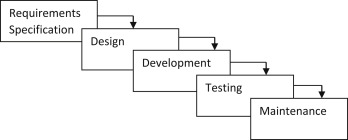
\includegraphics{waterfall}}
\caption{Software Development Lifecycle Using the Waterfall Model}
\label{waterfallfig}
\end{figure}
The classic approach to software development is to use a linear "Waterfall" methodology, stepping through all the essential parts of the software development lifecycle.
These key phases include the following: Requirements gathering, Design, Implementation, Testing, and finally Deployment/Maintenance.
Upfront, a timeline for the entire project is specified, allocating maybe 30\% of the project for planning, 40\% for coding the implementation, and the rest for testing/bugfixes and deployment.
Focussing on one complete phase at a time helps to ensure the entire product is cohesive and all the interacting parts have been designed with the whole project in mind.
This type of top-down approach works well when a project is routine, having well-understood requirements that are unlikely to change.

In general, the goal of a software engineering methodology is to minimize risk.
Conventional project management wisdom says that the closer that errors are found to when they were introduced means the least risk to the project's completion.
Conversely, the longer that an error persists, the greater the damage, with errors that make it into the release resulting in a product that either doesn't work or solves the wrong problem and wasn't what the client actually wanted.
A large disadvantage with the waterfall method is that errors in the design won't be caught until months or possibly years later when testing finally starts.
Catching and correcting design errors, even more so than difficult coding bugs can cost months of redesign and reimplementation.
For certain types of projects, it's very common for a client to realize that what they've asked for isn't what they really wanted only after seeing a completed product.
With the waterfall approach, where the client is only able to see the software after it's been fully implemented and tested, it's often too late or too expensive to make requirements changes.

\begin{figure}[tbh]
\centerline{\includegraphics[height=1.75in]{iterative}}
\caption{Software Development Lifecycle Using an Iterative Model}
\label{iterativefig}
\end{figure}
The spiral model was created to minimize risk by catching mistakes in the design and implementation closer to where they were introduced by producing multiple prototypes of the software.
The spiral model is an iterative approach as shown in Figure~\ref{iterativefig}, where we've taken the full waterfall lifecycle and repeated it on a small scale.
The spiral model also entails creating prototype of the full system from each cycle, even if many components are bare-bones or have to be mocked up.
The testing and evaluation of one iteration (or sprint) leads directly into the planning of the next iteration, allowing feedback to be taken on during development instead of after.
This also helps to catch problems with the integration and cohesion of different components that might not be found if end-to-end tests can't be run until the end of the project.
This is key to solving really hard problems where you're doing something that has never been done before, and it's often the case that the faster you fail, the faster you can succeed.
One possible disadvantage of the spiral method is that some effort might be wasted on prototyping components that much be re-written for the full implementation, but ideally the benefits of testing the full system outweigh this cost.

So, how does this all apply to an undergraduate dissertation undertaken by one a 1 person team?
Writing a compiler is a well-studied and understood task, with requirements documented by the project proposal that shouldn't change, which might lend itself to the waterfall method.
At the same time, the interactions between the components of a compiler can be complicated, with changes to the parser output greatly effecting code generator and vice versa.
The proposal is also specifying more like 1.5 projects, with the optional extension as an iterative addition to a finished base project.
The hard submission deadline with harsh penalties for being late also drove me away from a waterfall approach where errors found at the end of the project causing large delays are not acceptable.
So it made sense to me to use the spiral approach or creating a full compiler every few weeks with larger and larger subsets of OCaml until the base project and possibly extensions were finished.
Having a prototype of the compiler would also allow me to get better feedback from my supervisor with full demonstrations of progress.
Some effort was wasted prototyping components that would later be fully rewritten, but these the lessons learned from these prototypes were invaluable in writing the full compiler.

\subsection{Test Driven Development}
Test Driven Development (TDD) describes a broad set of practices with the common element that tests are written before what they're testing has been implemented.
This is often most effective when applied at the scale of unit tests, but can also apply to end-to-end tests as in the case of this project.
So, what are the benefits of writing tests first?
For a 1 person project like mine, writing your own tests can leave large blind spots.
If I've just spent days implementing some functionality, I can hardly test my implementation as if it's a black-box and edge cases missed in the implementation will likely be missed by the tests as well.
Writing tests is also in a sense part of the design process, forcing the programmer to consider the requirements of a component before they start coding.
Another benefit of having tests before you start coding is that you know you've finished once the tests all pass, and any extra work or refactoring is optional.
There's also the obvious benefit that you end up with lots of tests that are not just an afterthought, but can play an active part in the development process.

For these reasons, I started my project by writing the sample OCaml programs described above, adding tests for the expected output, and setting up automated end-to-end testing using the JavaScript test framework Mocha.
Having these sample programs was also invaluable for evaluating the compiler against JavaScript versions of the same programs and against the \JSofOCaml compiled versions.
I started the project by writing smaller unit tests for the parser and code generator, but did not keep up with this formal testing through development.

\subsection{Kanban Organizational Technique}

\begin{figure}[H]
   \centering
   \begin{minipage}{0.45\textwidth}
      \centering
      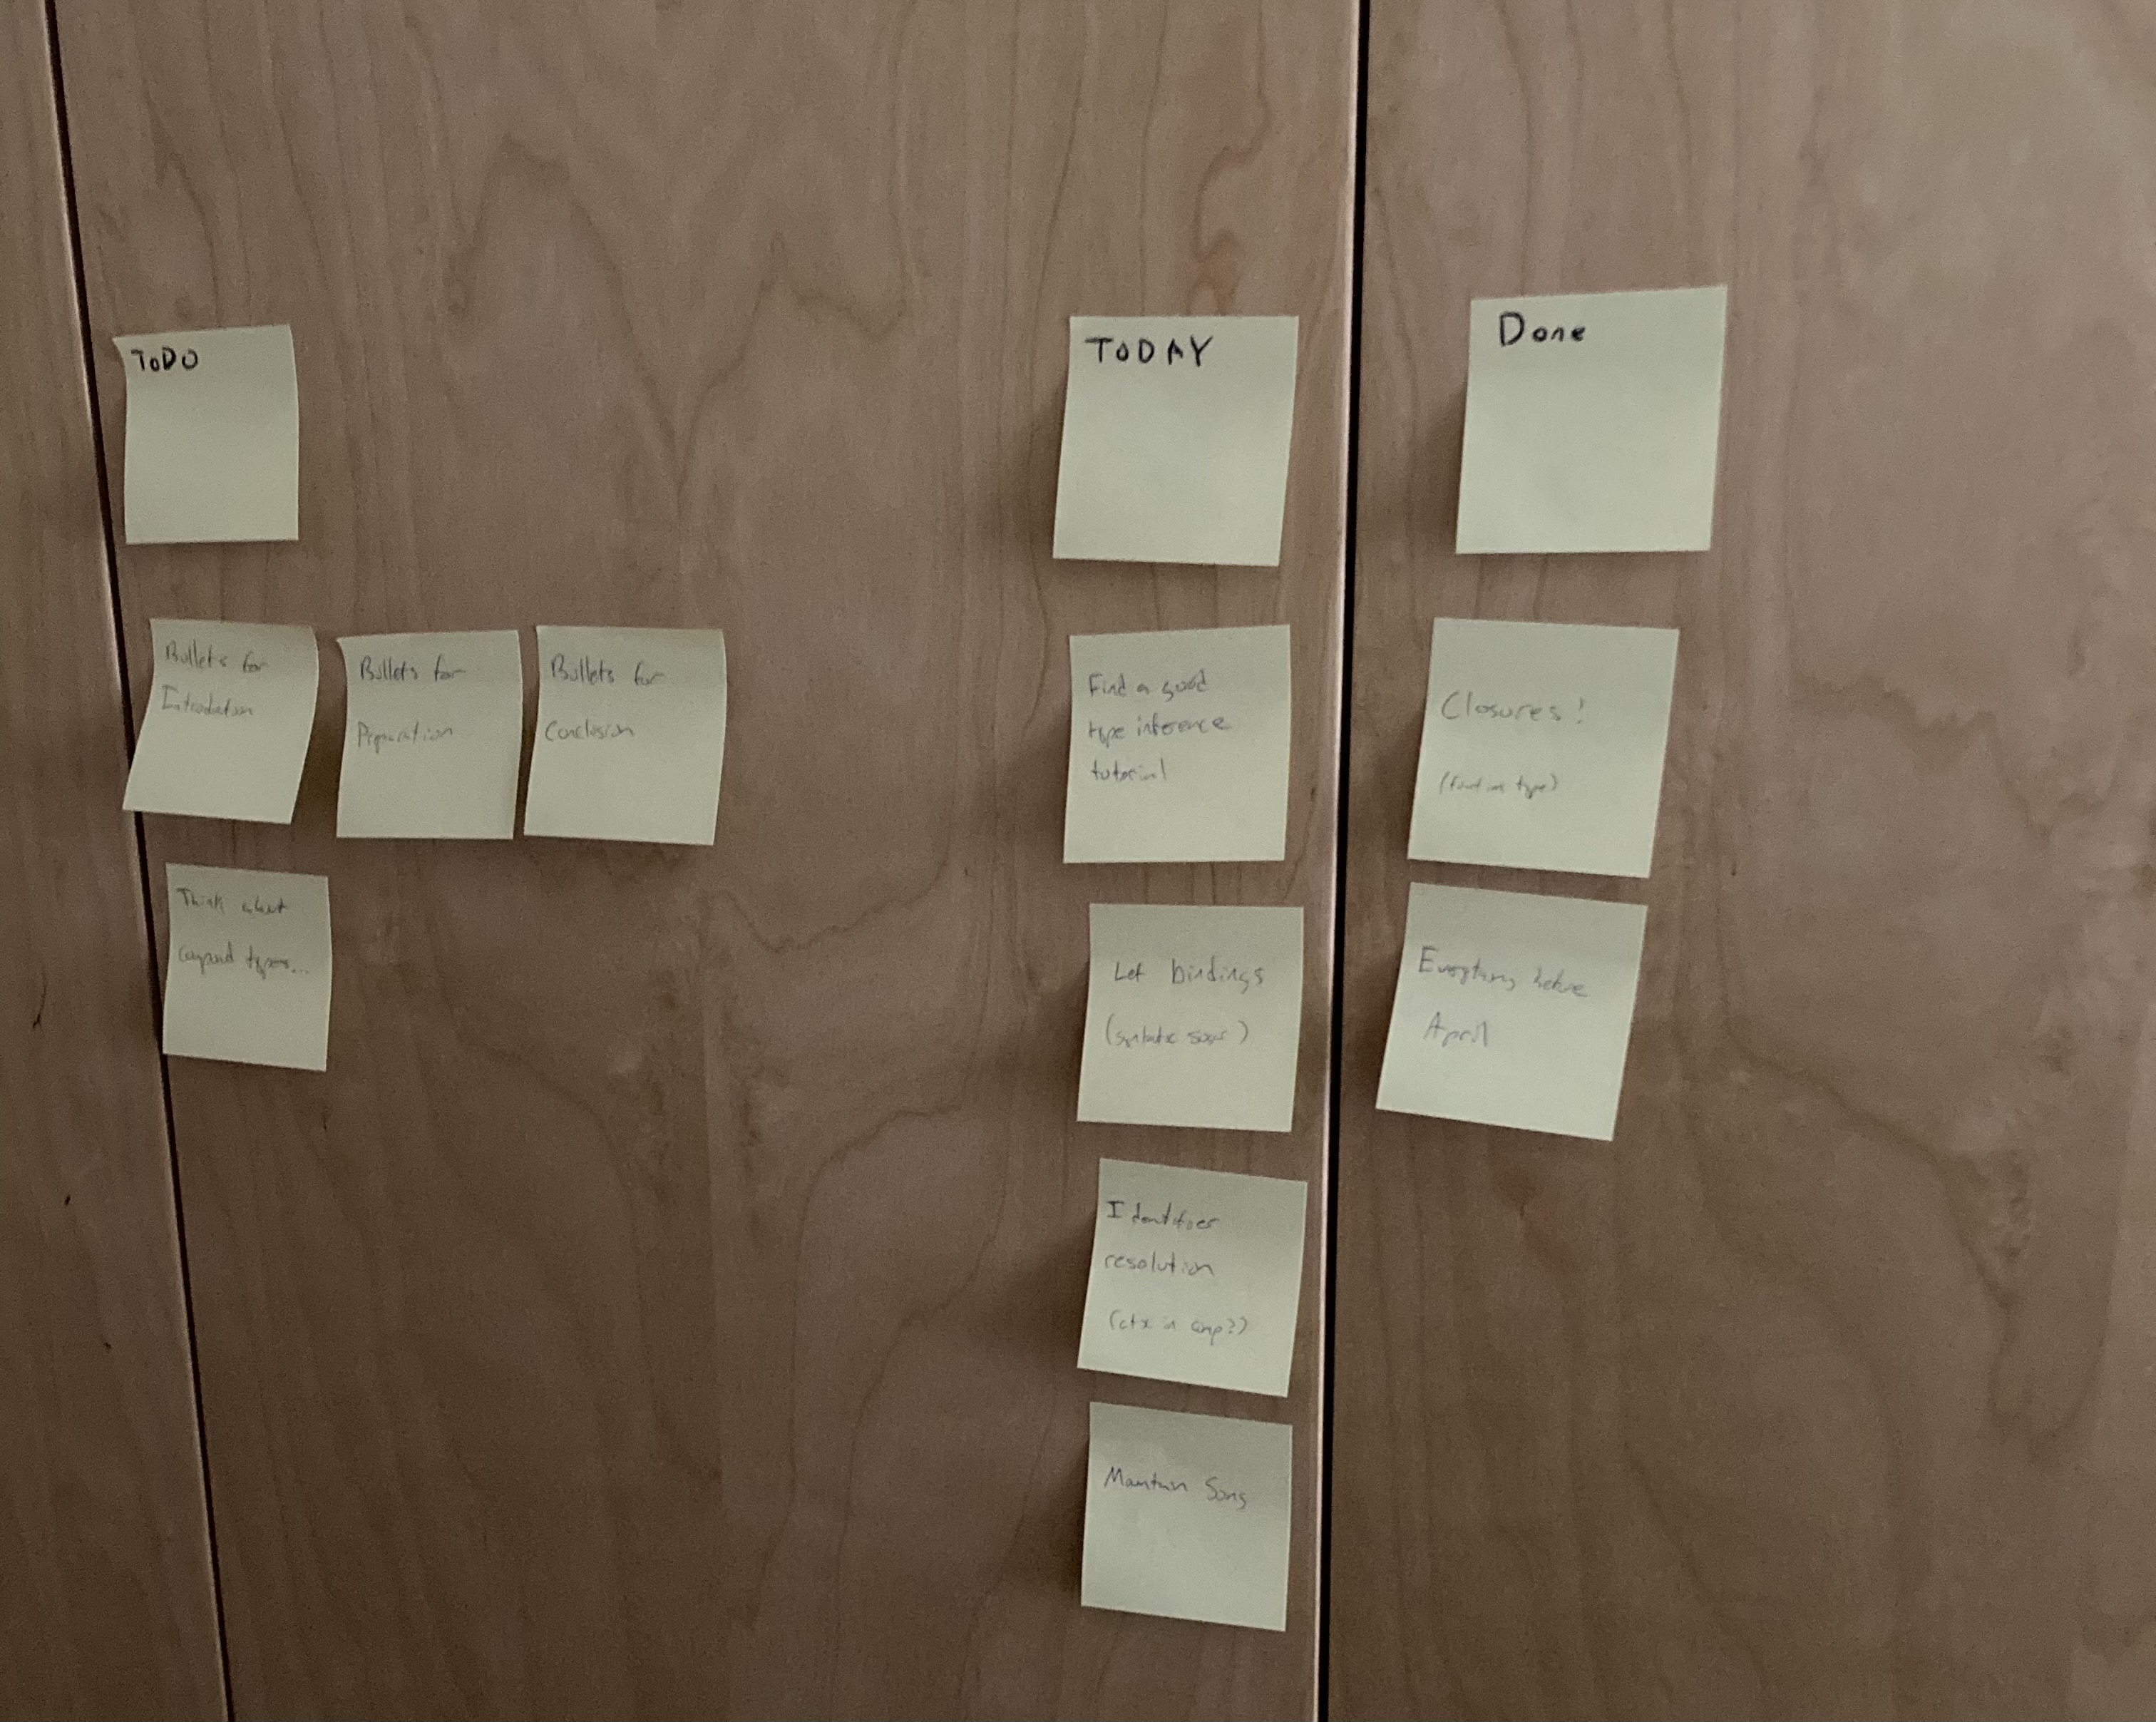
\includegraphics[height=1.5in]{kanban-early}
      \caption{The kanban board early in development}
   \end{minipage}\hfill
   \begin{minipage}{0.45\textwidth}
      \centering
      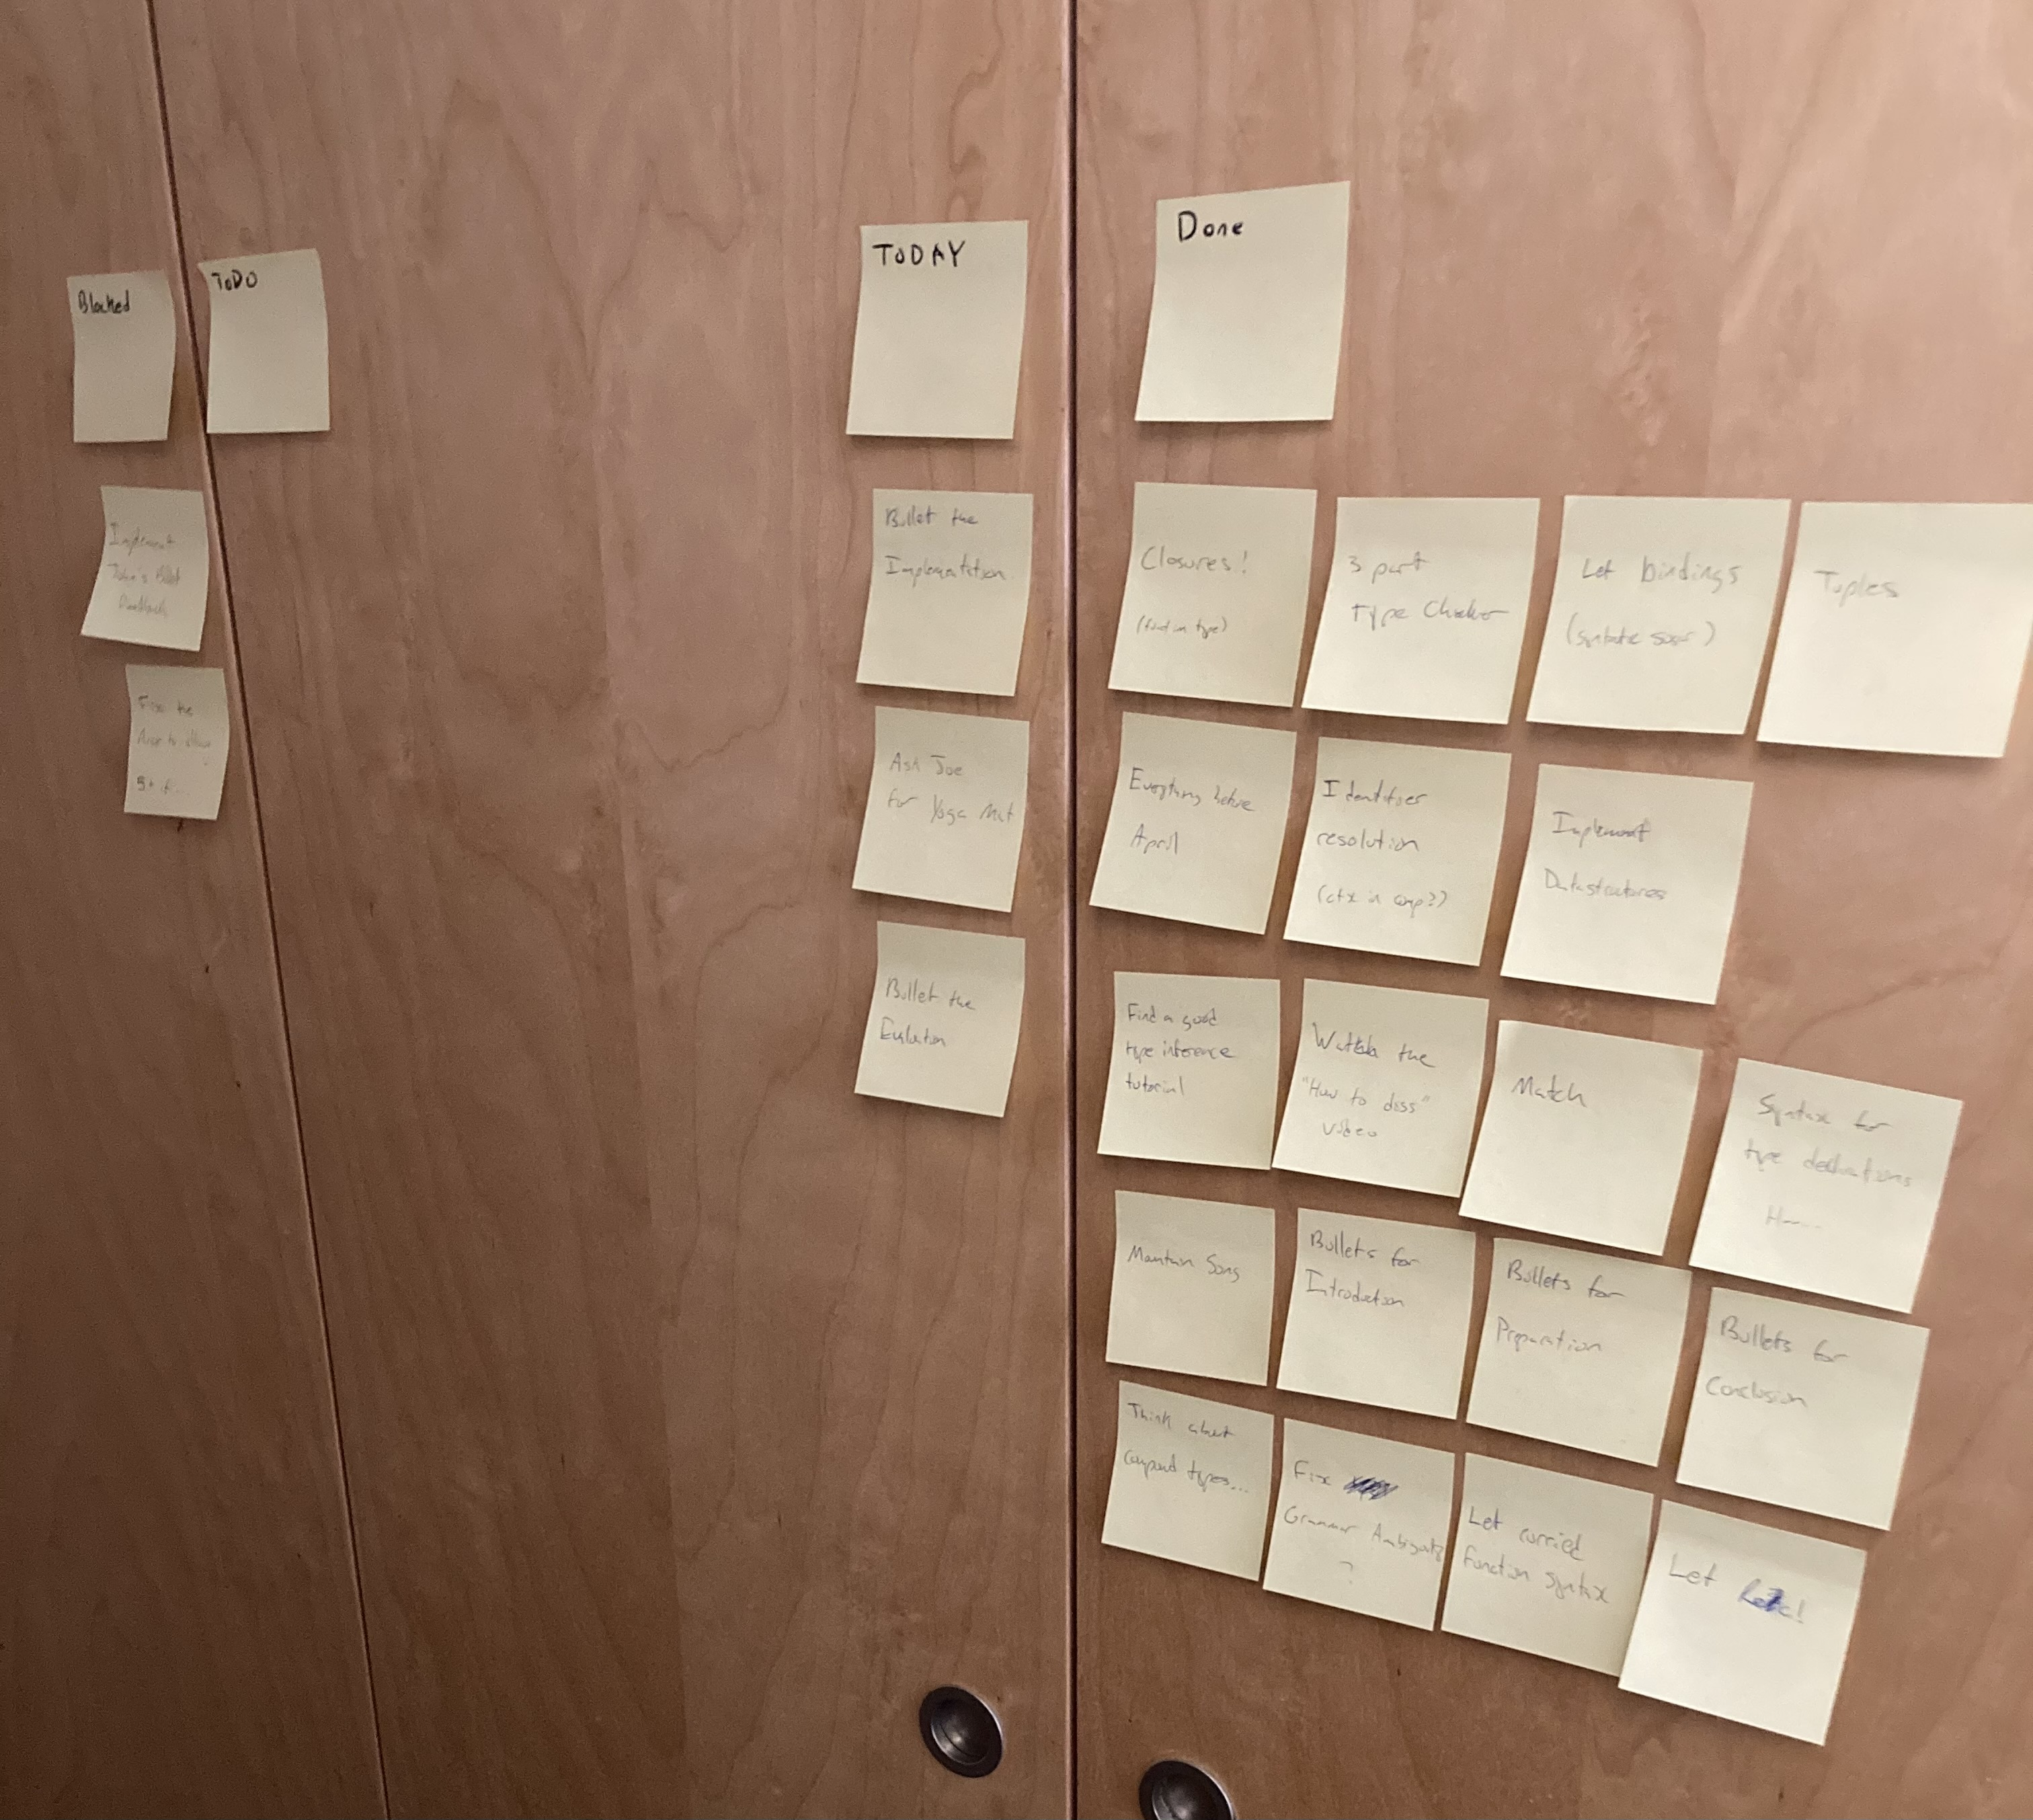
\includegraphics[height=1.5in]{kanban-late}
      \caption{The kanban board later in development}
   \end{minipage}
\end{figure}
Kanban is a popular method for managing workflows in software engineering.
It can be complicated or simple, but the important feature is you have a visual system for tracking tasks through your workflow.
For my project, this was a wall with sticky notes representing small tasks that needed to be completely for the project taking max a couple of hours.
Breaking the project into these small units is helpful for managing and tracking progress.
My board hard 4 columns: To Do, Today, Blocked, and Done.
At the start of an iterator (or a milestone from the project proposal), the To Do column should be filled with all the tasks necessary to reach finish this iteration's prototype.
Then on a given day spent working on the project, I would select a number of tasks proportional to the time I have to work and move them to the Today column.
If there was something blocking my progress, such as waiting for an answer to a question from my supervisor or another task needing to be completed first, that sticky note would be moved to the Blocked column.
Finally, completed tasks are moved to the done column.
Some of the organizational benefits of using kanban were lost because I'm not working on a team and the scope of the project was probably manageable without this tool, but it still served a purpose for my personal organization and juggling completing several tasks in parallel.

\subsection{Source Control / Backup}
Git was used for both source control with Github as a remote host and backup solution.
Backup was important for this project in the unlikely case that something happens to the files on my local machine, I won't lose all progress.
The project is publicly hosted on github and can be downloaded in the case of disaster.
Git was a necessary tool on this project for tracking changes to the source code and organizing those changes in to meaningful commits.
Commits then become the tangible unit for thinking about progress on the project allowing us to checkout a commit to see a snapshot of the project at a certain point, remove a commit from the history to undo a set of errant changes, or organize the project into branches of related work to be developed in parallel.
The collaborative benefits of Git and Github weren't realized by this work on the project, but could be used in future efforts to improve the compiler.

\chapter{Implementation}

\section{Repository Overview}
\subsection{Filestructure}
\dirtree{%
.1 Wasm\_of\_OCaml/.......................2104 LOC.
.2 docs/...............................0 LOC.
.2 learn/............................363 LOC.
.2 src/.............................1377 LOC.
.3 ocaml.jison....................260 LOC.
.3 parser.js.......................49 LOC.
.3 transform.js...................248 LOC.
.3 typer.js.......................315 LOC.
.3 comp.js........................325 LOC.
.3 main.js........................179 LOC.
.2 test/.............................364 LOC.
.3 samples.test.js.................56 LOC.
.3 run-experiments.js..............68 LOC.
.3 samples/.......................142 LOC.
.4 8-queens.ml..................19 LOC.
.4 ...11 other sample.
.3 ocaml/..........................49 LOC.
.3 js/.............................30 LOC.
.3 js\_of\_ocaml/.....................0 LOC.
.2 package.json.......................0 LOC.
}

\begin{figure}[tbh]
\centerline{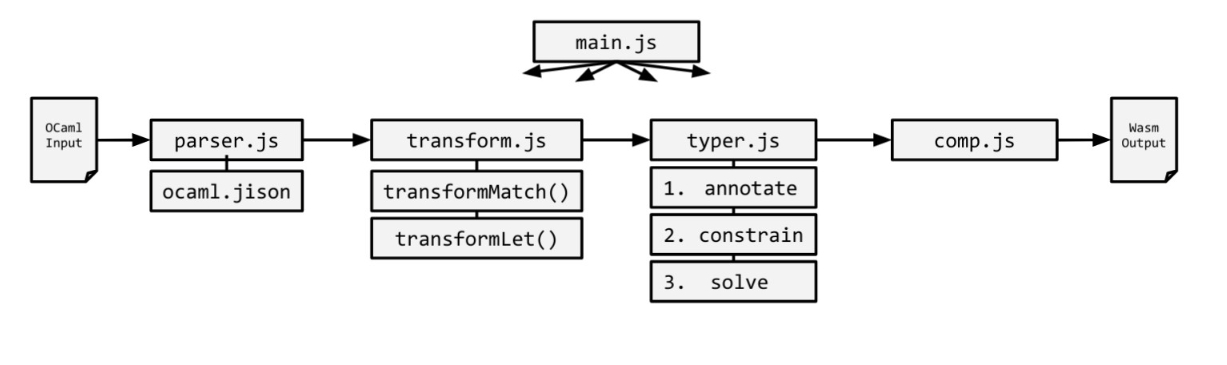
\includegraphics[height=2in]{pipeline}}
\caption{Diagrammatic view of the compiler}
\label{pipeline}
\end{figure}

\subsection*{{\tt docs/}}
The {\tt docs/} directory contains important documents for the project including this dissertation.

\subsection*{{\tt learn/}}
The {\tt learn/} directory contains code that I experimented with related to the project, but aren't a part of the source.
For example, to get familiar with WebAssembly, I implemented conway's game of life, and that code lives in the learn directory.

\subsection*{{\tt src/}}
The {\tt src/} directory contains all the code for the compiler.
{\tt main.js} is the entrypoint to the code, exporting a function {\tt compileAndRun(src)} which returns the result of compiling and executing (in Wasm) an OCaml program.
{\tt logger.js} exports a logging function used by all the other files, which can be modified to reduce the amount of debug statements flooding stdout.
The rest of the files and how they relate to eachother is shown in Figure~\ref{pipeline}.

\subsection*{{\tt test/}}
The {\tt test/} directory contains the code for evaluating the compiler.
There are to toplevel files scripts for evaluation: {\tt samples.test.js} which runs end-to-end tests on the 12 sample programs and {\tt run-experiments.js} which takes performance measurements on the 9 performance tests.
{\tt samples/} contains the 12 OCaml programs as inputs to the compiler for the end-to-end tests.
There are 3 directories each containing 3 programs for the performance tests: iterative Fibonacci, recursive Fibonacci, and quicksort.
{\tt ocaml/} contains the OCaml versions to be compiled by my compiler.
{\tt js/} contains the handwritten JS versions to be run with Node.
{\tt js\_of\_ocaml/} contains the JS files generated by \JSofOCaml using the programs in {\tt ocaml/} as input.
Code in this directory was not included in the line count because it was about 6000 lines of generated code.

\section{Parsing}
For parsing, I've used the powerful Jison port of the parser generator Bison.
This means all the information for parsing is in the {\tt ocaml.jison} file and {\tt parser.js} is just an interface that works with Jison.
I could have used Jison to generate JavaScript source files for a parser, but to allow quick changes to the parser for ease of development, a parser object is generated by Jison each run of the parser.
For a full release though, it would be simple to generate a parser once, and just include that parser in the source of the project.

\subsection{Lexing}
The first stage of the front-end of a compiler is usually the lexer, which groups smaller chunks of characters in the source code into tokens.
Grouping and classifying raw characters in the source can be done using regular expressions, instead of the more powerful context-free grammars for full parsing.
OCaml is white-space insensitive, so the lexer also discards whitespace characters.
This was a simple task as patterns for tokens are described in the OCaml spec. \\
Here are a few example rules for lexing:
\begin{itemize}
   \item {\tt /"-"?[0-9][0-9\_]*/g return 'INT\_LITERAL'}
   \item {\tt /"true"|"false"/g return 'BOOL\_LITERAL'}
   \item {\tt /[a-zA-Z\_][a-zA-Z\_0-9']*/g return 'ident'};
\end{itemize}
The parser will then deal with grammar symbols and tokens such as {\tt 'INT\_LITERAL'} and {\tt 'ident'} as terminals.

\subsection{The Grammar}
The grammar is pretty straightforward with top-level declarations for the important units of a program such as: {\tt expr}, {\tt type-decl}, and {\tt pattern}.
There are then many more grammar symbols for implementing these higher level language features.
Much more important than determining whether a string is in the language is constructing the parse tree.
As we'll see throughout this chapter, our AST is a normal JS object with each node in the tree having a {\tt tokenName} property such as {\tt 'LET'}, {\tt 'INFIX\_OP'}, or {\tt 'FUNC'}.
Along with a tokenName, a node will have properties dependant on the token type, including the objects for child nodes and sub-expressions.
Jison lets us specify code along with a grammar rule, allowing us to construct an object when that rule is reduced, and giving us access to what's been produced by the components of the rule.
As an example, here is the rule for a non-recursive let expression:
\begin{verbatim}
expr:
   'let' let-binding 'in' expr
      {$$ = {tokenName: 'LET', rec: false, binding: $2, body: $4}} \end{verbatim}
\subsection{Resolving Ambiguity}
A direct translation of the grammar in the OCaml specification results in a grammar that's context free, but not in $LR$. We get lots of constructions like the following:
\begin{verbatim} expr:
   expr '+' expr
 | expr '*' expr
 | expr '||' expr \end{verbatim}
This grammar results in many shift-reduce conflicts while constructing the parse table.
My first try at resolving this ambiguity was to annotate the rules to force the parser into making certain reduce decisions when there's a conflict.
We can give Jison an ordered list of annotations such as {\tt \%left '+' '-'; \%left '*' '/' 'mod'}.
The keyword {\tt \%left} (or {\tt \%right}) gives the associativity of the operator and the order gives precedence, so in our example {\tt '*'} binds more tightly than {\tt '+'}.
This method was sufficient in the first few prototypes of the compiler, but I ran into a problem when implementing function applications.

Function application in OCaml is done using the juxtaposition of two expressions.
Unfortunately the rule {\tt expr: expr expr} introduces ambiguities that are not so easy to resolve.
The problem arises from the fact there is no separator between or around the expressions.
While we can give the precedence of this reduction, we cannot give the associativity of a blank operator in Jison.
The rules for expressions (and other constructs using juxtaposition) would have to be rewritten to grammatically fix this ambiguity.
So, the current version of the compiler has the precedence and associativity of operators encoded in the rules themselves.
The new grammar is structured something like this:
\begin{verbatim}
add-expr: mult-expr   | add-expr '+' mult-expr;
mult-expr: unary-expr | mult-expr '*' unary-expr;
unary-expr: app-expr  | '-' unary-expr;
app-expr: val-expr    | app-expr val-expr;
\end{verbatim}
After trying lots of different things with precedence annotations and being stuck on the ambiguity of the juxtaposition operator for a while, switching to this style of grammar worked right away and solved so many problems.

\section{Code Transformations}
A design decision I made was to keep the backend (type inference and code generation) as simple as possible.
There were some redundant language features so useful and convenient that they were essential even in my small subset of OCaml.
Rather than handling these constructs which are almost syntactic sugar throughout the compiler, I chose to translate them to simpler constructions directly after parsing.

\subsection{Match Translation}
Pattern matching is one of the more useful and unique features of OCaml, which has no good analogs in JavaScript.
A {\tt match-with} expression can be decomposed into a set of tests checking whether a pattern has been matched, as well as let declarations for binding identifiers matched in the pattern.
Rather than implementing these checks and declarations at the code generation stage, I chose to translate {\tt match} expressions directly after parsing.

The helper function {\tt unifyPattern(pattern, matcher)} does the key work for translating pattern matching into {\tt IF} and {\tt LET} expressions.
{\tt unifyPattern} returns an object with two lists: a list of boolean expressions checking if the pattern has been matched and a list of let-bindings for variables declared in the pattern.
This function is designed for recursion because to match a tuple-pattern we must recursively match elements of the tuple with sub-expressions in the pattern, accumulating checks and declarations along the way.
Similarly, to unify a type-constructor pattern with a matcher, we need to add a check that the matcher was constructed with that type-constructor and then recursively unify the argument of the pattern with the argument extracted from the matching expression.

With sets of checks and declarations for each pattern, we can translate a {\tt match} expression as follows:
\begin{verbatim}
match e with
   pattern1 -> body1
 | pattern2 -> body2
\end{verbatim}
is translated to:
\begin{verbatim}
if check-1-for-pattern1 and check-2-for-pattern1 and...
   then let decl-1-of-pattern1 in
        let decl-2-of-pattern1 in ...
      in body1
   if check-1-for-pattern2 and check-2-for-pattern2 and...
      then let decl-1-of-pattern2 in
           let decl-2-of-pattern2 in ...
         in body2
      else throw match error
\end{verbatim}

\subsection{Let Translation}
Instead of having multiple ways to declare variables, I chose to carry only variables defined in functions forward into the back-end of the compiler.
This translation is based on the observation that {\tt let x = 2 + 2 in x * x} can be rewritten as {\tt (fun x -> x * x) (2 + 2)}
Let also gives us some extra syntax for defining functions and functions with multiple parameters.
But this can also be translated into function application with {\tt let f x y = x + y in f 2 3} being translated (slightly tediously) into {\tt (f => f 2 3) (fun f -> fun x -> fun y -> x + y)}.
So translating let expressions into function applications, is quite straightforward and only requires some re-arranging and explicit currying for function declarations.

These two translations for match and let allow us to extend the syntax of the language without having to add additional cases to the type inference algorithm or the code generator, which would be a significant amount of work.
Instead, we can piggy-back off already implemented code for function application and {\tt if-then-else}.
\section{Type Checking/Inference}
For type inference, I've used a 3 phase constraint-based approach resembling some of the data-flow analysis algorithms taught in the part II optimising compilers course.
This resemblance makes sense because type inference can be considered a data-flow analysis, where the flow of types is based on the semantics of the OCaml type rules.
The 3 phases of the type inference algorithm are as follows: annotate, constrain, solve.

\subsection{Annotate}
Annotation is the simplest phase, whose role is to give every node in the AST a type-variable which will later be replaced by a concrete type.
This is almost as trivial as traversing the AST object and adding a {\tt "type"} property with a uniquely generated type-variable to each node.
The only complication is that instances of the same identifier should have the same type-variable.
To accomplish this, we keep track of an environment, and every time a new identifier is declared, a new type-variable is generated and added to the environment attached to the new variable.
Then when an we are annotating an identifier, we look-up it's type-variable in the environment.
If the identifier is not found, then we report an error because this identifier has not been declared.
\subsection{Constrain}
In the constrain phase, we use the typing rules of the language to generate constraints on the types in the AST.
A constraint is represented by a pair of types which must unify with each other.
In the simplest case, where we are constraining the expression {\tt \{tokenName: "INT\_LITERAL", type: "t13", val: 42\}}, we would generate the constraint pair {\tt ("t13", "INT")}.
As another example, if we have a function application {\tt app}, where that application has a {\tt func} and an {\tt arg}, we would generate the following constraint pair: {\tt (func.type, \{type: 'FUNC', fromType: arg.type, toType: app.type\})}.
Generating these constraints correlates exactly with applying rules in the formal type system.
So, to generate all the constraints, we traverse the AST accumulating these pairs for each node in the AST, with some nodes such as {\tt if-then-else} generating multiple constraints.

\subsection{Solve}
The final step in our algorithm is to solve the system of constraints and associate a concrete type with each type-variable generated in the annotate stage.
With this solution, we can substitute the concrete types back into the AST.
Our solution takes the form of a map from type-variables to types.
Below is algorithm for generating a solution from a set of constraints:
\begin{enumerate}
   \item Initialize the solution to an empty map.
   \item Repeat for each constraint.
      \begin{enumerate}[i.]
         \item Apply the substitutions in the current solution to update our constraint.
         \item Unify the two sides of the constraint to generate a set of new substitutions.
         \item Apply the new substitutions to our current solution.
         \item Add new substitutions to the solution if they didn't exist.
      \end{enumerate}
\end{enumerate}
Two subroutines of the above algorithm are unifying two types and applying a set of substitutions to a type.
Unification is done with the classic unification algorithm, recursively unifying two types and generating a substitution when type-variables are found.
If the types can't be unified, then the constraints have no solution, and therefore the program has a type error, which we can report.
Substituting a solution map into a type is also as simple as traversing the type looking for type-variables that are in our solution and doing a lookup.

\subsection{Polymorphism}
The above algorithm is already nearly equipped to handle polymorphic types.
If there a type cannot be constrained to a concrete type, the algorithm will end up with type variables which for the polymorphic types.
However, significant work would have to be done on the code generation side to accommodate polymorphism.
For that reason, our subset of OCaml does not support polymorphism.

There is however, a bit of polymorphism to comment on within the type inference algorithm.
Our subset of OCaml includes comparison operators which operate on several comparable types, as well as match-errors which can take any type.
For these constructs, there are two special types {\tt 'COMP'}, which unifies with {\tt 'INT'}, {\tt 'FLOAT'}, and {\tt 'BOOL'} types as well as the {\tt 'ANY'} type which unifies with every type.
Some care must be taken in the constraint-solving phase that a type should take on the most specific type which we have found for it.

\section{Code Generation}
Code generation is the final stage of compilation, taking transformed and typed AST and producing executable Wasm code in the {\tt .wat} format.
Code generation all runs through one function in {\tt comp.js} conveniently also called {\tt comp}

First, I'll describe the {\tt comp()} function's signature, and then we can dive into how it works.
There are 3 parameters: {\tt ast}, {\tt ctx}, and {\tt depth}.
AST is self-explanatory and ctx and depth are used to generate code for looking up variables in the context/environment.
There are also 3 values returned from compiling an expression: {\tt code}, {\tt defs}, and {\tt localDefs}.
{\tt code} is the code that computes the expression, {\tt defs} is a collection of function definitions needed to execute the code, and {\tt localDefs} is code for defining local variables used by the code.
{\tt localDefs} is returned separate from the code because local definitions must appear at the beginning of a Wasm function.

Generating stack based code for the basic operations is quite trivial.
For a {\tt '+'} expression, we recursively take the code for the left subexpression, append the code for the right subexpression, and then append the line "{\tt  i32.add}".
The two values computed by the sub-expressions will be left on the top of the stack and the add instruction will add pop the top two values and push back on their sum.

Generating code for more complicated expressions requires support from additional data structures and helper functions.
This code and data that accompany the generated code is our runtime, which for our compiler is about 70 lines of WebAssembly added to every compiled file.
Our runtime mainly assists programs with doing two things: allocating memory on the heap and creating and applying functions.

\subsection{Memory Management}
For memory management, we have a very simple bump allocator.
There are proposals for extending WebAssembly to have garbage-collecting features, so in the future more sophisticated memory management might be possible without too much modification of our compiler.
But for now, we allocate a piece of memory for our runtime heap, which can be accessed from the outside JavaScript.
Exposed internally is a global variable {\tt \$heap\_ptr} which points to the next free byte on the heap.
Bytes on the heap can be interpreted either as {\tt i32}s or {\tt f32}s, and because OCaml is strongly typed, we always know the type of data we've stored.

Besides our 3 primitive types, we have 3 heap-allocated types: functions, tuples, and datatypes.
We'll look at tuple and datatype creation now and show how functions are implemented in the next section.
Values of every type conveniently take up 4 bytes (1 word for our case), either as a direct value or a pointer onto the heap.
To construct an n-tuple, we simply allocate n words on the heap, store the top n-values on the stack into our tuple, and lastly push the address of the tuple onto the stack.
To project from a tuple, we simply load from the heap at the appropriate offset from the tuple's value.
Datatypes are nearly a special case of tuples where the index of the constructor used is stored on the heap along with the constructor's argument.
When a constructor is used in a pattern-match, we load the first word from the 2-tuple and compare it to the fixed index of the constructor.
To extract the constructor's argument, we simply load the second word.

\subsection{Functions and Closures}
To implement a functional language OCaml, function pointers and indirect calls are essential.
Luckily WebAssembly allows us to declare a funcref table and do indirect calls to functions in that table.
Each function in the collection of function definitions returned by {\tt comp()} adds its function to the top-level and adds an entry to the function table.
Function values are represented by closures, which are a pair consisting of an index into the function table and an environment pointer.
Closures get their name because a function value closes over the variables in it's environment at the time of it's creation.
Without this feature of functional languages, important techniques like currying would not be possible because a function wouldn't save the state of surrounding variables at its creation.
In our implementation, the environment is a linked-list containing the value of every variable up to the root which has no defined variables.
The syntactic depth of a function expression is the same as the length of this environment list because that is the number of variables accessible at the time of function creation.
By syntactic depth, I mean the number of function definitions surrounding the code in the source program.
This relies on the fact that OCaml functions have exactly 1 formal parameter.

The environment linked-list accessible with every function is the reason for the {\tt depth} argument of {\tt comp()}.
The current syntactic depth, as well as the depth of each variable needs to be kept track of so that we can traverse the environment list to get a variables value.
The {\tt ctx} variable to {\tt comp} contains a map from identifiers to the depth of the function declaring that variable.
For example, if we are looking up an identifier declared at depth 3 and we're currently at depth 5, then the code generated to access that variable must traverse back 2 nodes on the environment list.
So, when compiling a function expression, we must add the function parameter's identifier to the context with it's value as the current depth and increase the depth by 1 when compiling the function's body.
When the function looks up it's own argument's value, it doesn't have to follow any pointers in the environment list, it only has to load the value from the first node.

To apply a function value to an argument, we need to allocate a new node in the environment list to store the argument's value.
That new node points to the function's environment as the rest of it's linked-list.
To call the function, we extract the index into the funcref table from the closure and do an indirect call using that index with the environment list as the argument.
WebAssembly handles all the work managing the call-stack and leaving the result of the called function on the stack after it returns.

The last piece of the puzzle to address is recursive functions.
Recursive functions can only be declared with a {\tt let rec} binding.
In the translation stage where let bindings are transformed, a metadata is added to the definition of a recursive function, which marks a function as recursive and notes the identifier it has to refer to itself.
This information is also used in the type algorithm while adding identifiers to the context there.
To give a recursive function access to its own closure, we add an element to the environment list for that function.
This addition to the environment is also reflected in the {\tt ctx} and {\tt depth} parameters of {\tt comp()}.
Whenever a closure of a recursive function is created, we just allocate an extra node on its environment list with the function's index in the funcref table.
This addition of an extra variable lets us have single-recursive functions (our subset of OCaml does not include mutual-recursion, although it would be possibly by adding multiple entries to the environment).

\chapter{Evaluation}

Does the compiler really work?
How do programs compiled by my compiler compare to alternatives for writing the same program?
In this chapter, we aim to answer these questions by first detailing the methods used to evaluate the compiler.
Then, we will analyse the data produced by our experiments.
Finally, we will synthesize these results to answer the question: did this project meet it's success criteria?

\section{Evaluation Methods}
At a high level, we will evaluate the compiler by writing OCaml programs, compiling them, and testing the  correctness and performance of the resulting WebAssembly.
\subsection{Extended Sample Programs}
The sample programs described in the project proposal and preparation chapter were used as end-to-end tests of the compiler.
In order to test the compiler more thoroughly and better isolate behaviors, an additional 7 sample programs were developed.
\begin{multicols}{3}
\begin{itemize}
\itemsep-.2em
\item Int Arithmetic
\item Float Arithmetic
\item Boolean Arithmetic
\item 8-th Power
\item Factorial
\item Recursive Fibonacci
\item Iterative Fibonacci
\item Integer Square Root
\item Euclid's Algorithm
\item FizzBuzz
\item Quicksort
\item N-Queens
\end{itemize}
\end{multicols}

\subsection{9 Performance Programs}
In addition to end-to-end testing the compiler for correctness, we will evaluate the compiler by comparing it to two alternatives methods of executing an OCaml program on the web.
The two alternatives are to compile the OCaml to JavaScript using the \JSofOCaml tool or to handwrite a JavaScript version matching the OCaml.
\JSofOCaml works by taking bytecode produced by a full OCaml compiler and translating that bytecode into JavaScript.
Because the code is first compiled by the OCaml compiler, we can expect optimizations like tail-call optimizations to be applied.
Even with optimizations, I would expect idiomatic, handwritten JavaScript to outperform this generated JS.
Both compilers will benefit from JavaScript optimizations done by the V8 engine as it JIT compiles our code.

We will use 3 programs to compare the different methods: recursive Fibonacci, iterative Fibonacci, and Quicksort.
By recursive Fibonacci, I mean the top down translation of the formula $fib(n) = fib(n-1) + fib(n - 2)$ as opposed to the iterative implementation which computes Fibonacci numbers up to the target.
The recursive implementation is meant to be inefficient and doesn't include any memoization to improve the complexity.
Also, by when I say iterative Fibonacci, the solution is still uses recursion (imperative loops have not been implemented), I just mean that it's tail recursive and computes Fibonacci numbers bottom up.
The quicksort implementation is also no frills quicksort using the first element as the pivot and without augmentations like in-place quicksort.
The JavaScript version is made to resemble as closely as possible the OCaml version, except that it uses builtin JS arrays (but it does not modify them).

These programs were chosen to each have a different time complexity with recursive Fibonacci being $O(2^n)$, iterative Fibonacci being $O(n)$, and Quicksort being $O(n\log{}n)$.
There will be 9 programs in total, solving the 3 problems using each of the compilers.

\subsection{Timing the Programs}
In order to gather our data, we need to time programs in each of the 3 different styles.
This proved harder than initially thought because it's important that only the runtime of the functions are included and not setup and teardown that happens around that execution.
For both the Wasm execution and the handwritten JavaScript version, we were able to use JavaScript's performance timer which gives timings in nanoseconds.
However, for the \JSofOCaml version, we can only access the OCaml timing functions, which only give us millisecond precision.
Normally, it wouldn't be a problem because we could use milliseconds for both, however the timing programs all execute in about 1-5 milliseconds.
The source of the problem is that my WebAssembly compiler doesn't do any garbage collection, and additionally every function call allocates a new node on the environment list for a functions parameter.
So, without any optimizations such as tail-call optimizations, programs processing large inputs end up filling up memory quite quickly.
For this reason, we can't just run the tests on larger inputs to get longer times, and must deal with the low-precision millisecond timings for the \JSofOCaml tests.

\section{Results}
\subsection{Iterative Fibonacci}
\begin{figure}[tbh]
\centerline{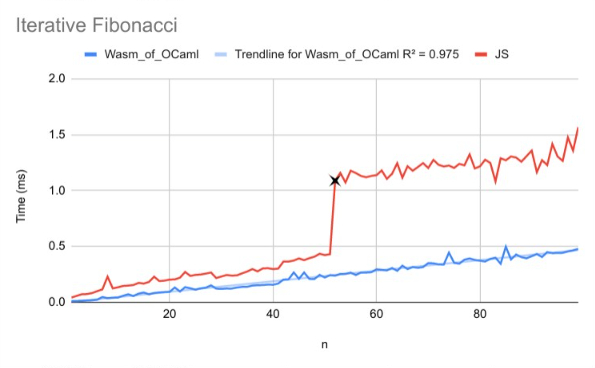
\includegraphics[height=2in]{fib-iter-graph}}
\caption{Execution time of iterative Fibonacci}
\label{fib-iter-graph}
\end{figure}
As we can see in Figure~\ref{fib-iter-graph}, our WebAssembly compiler computes Fibonacci numbers about twice as fast as a handwritten JavaScript implementation.
This is a good speedup especially considering there are no optimizations done on the WebAssembly, not even tail-recursion reduction which would greatly improve performance.
At the same time, this shouldn't be too much of a surprise considering WebAssembly is much closer to a native instruction set.

The WebAssembly runtime growth looks very linear as we should expect, with an $R^2 = 0.975$ for the line of best fit.
The JavaScript graph is quite linear as well, except for the large jump around $n=50$.
This sudden jump from one linear progression to a different one was quite puzzling, but there's a solid explanation, which relates back to the motivation of this project.
The slowdown comes right after we try to compute $fib(49) = 4807526976$, which just so happens to be the first fibonacci number which overflows signed 32 bit integers, which are part of what JavaScript uses to represent it's {\tt Number} type.

So why does hitting 32-bit overflow cause a slowdown for JavaScript and not WebAssembly?
It's not because WebAssembly uses 64 bit integers, which would be possible, except my implementation uses {\tt i32}.
When JavaScript a Number value has overflowed, it converts that Number to a float and proceeds with floats for the rest of the program.
So, we get a slowdown after $n=50$ because from that point out JavaScript is doing slower floating point arithmetic.

This JS behavior is yet another example of JavaScript's type system surprising us and coercing types while we're not looking to avoid errors.
While in some cases automatically switching to use float representations might be very convenient and avoid bugs due to integer overflow, it can equally cause difficult to identify bugs.
Once a Number has switched to using a float representation, using it in any arithmetic expression will coerce the other operand to be a float too and result in a float.
This would be acceptable if floats were a subtype of integers, however there are many strange properties of floats that integers don't have.

\subsection{Recursive Fibonacci}
\begin{figure}[tbh]
\centerline{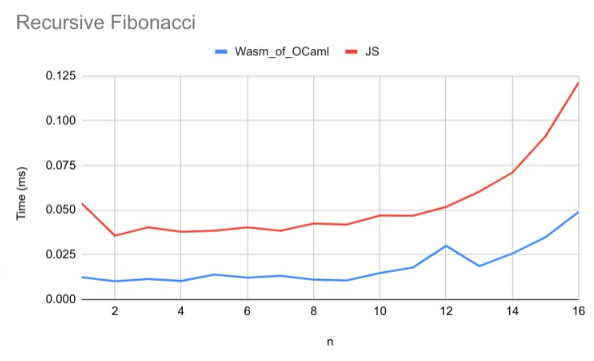
\includegraphics[height=2in]{fib-rec-graph}}
\caption{Execution time of recursive Fibonacci}
\label{fib-rec-graph}
\end{figure}
The recursive Fibonacci program suffers from the memory problem that prevents us from running it on large inputs.
This is especially true for the recursive version because the recursive function calls branch and grow exponentially.
That's why we could only run this up to $n=16$.
Still, these 16 datapoints can tell us something about our compiler.
There are two things to notice.
First is that our {\tt Wasm\_of\_OCaml} compiled version still has a 2-3x speed advantage over the handwritten JavaScript running on V8.
The other thing to notice is that within the small sample size, both curves fit the expected exponential growth.

\subsection{Quicksort}
\begin{figure}[tbh]
\centerline{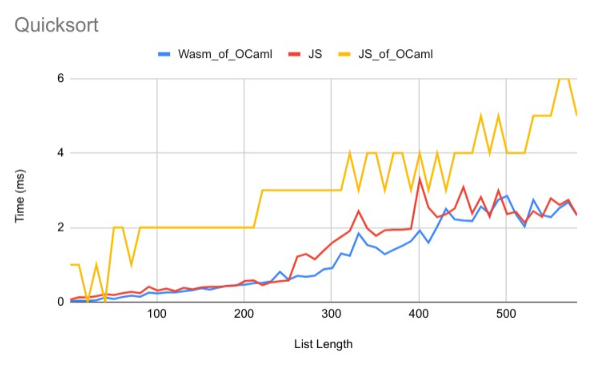
\includegraphics[height=2in]{quicksort-graph}}
\caption{Execution time for quicksorting a shuffled list}
\label{quicksort-graph}
\end{figure}

The runtimes for quicksort were long enough without running out of memory that I was able to include the results from \JSofOCaml in Figure~\ref{quicksort-graph}.
Here, the performance of our compiled Wasm code is quite similar to the JavaScript implementation.
While it's faster for most lists, there are some inputs where the handwritten JavaScript outperforms it.
One reason for this may be that our OCaml implementation defines its own linked list datatype as well as operations on those lists, whereas JavaScript uses faster arrays with better optimized array functions.
This is the largest program of the 3, so it's also possible the speed loss from not having any optimizations is greater for more complex programs.
As we expected, \JSofOCaml is strictly slower than our handwritten JavaScript by a decent margin, although the lack of resolution makes it hard to compare.

The relatively small number of tests and the high variability makes it difficult to draw conclusions about the shapes of the curves.
A large part of the jaggedness is inherent in the quicksort algorithm, which is only $O(n \log n)$ in the average case.
All 3 programs are run on the same randomized list for each input size, so the comparison is fair in that way, but the variation in how well the pivot divides the list in 2 makes it harder to fit a trend line.
We can still conclude that it looks as if all 3 programs have similar time complexities that could follow a linearathmetic progression.
In hindsight, mergesort may have given more stable and informative results.

\section{Success Criteria}
\begin{figure}[tbh]
   \centerline{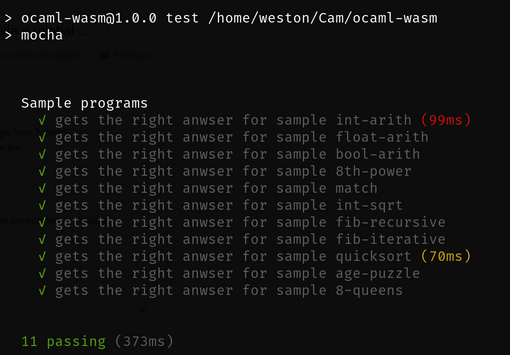
\includegraphics[height=2in]{passed-tests}}
\caption{Output from the mocha end-to-end test suite showing 12/12 passed}
\label{passed-tests}
\end{figure}
From the project proposal, my success criteria was to show the compiler correctly compiles programs within the subset of OCaml into WebAssembly.
The set of 12 sample programs certainly uses every feature in our small subset of OCaml and as Figure~\ref{passed-tests} shows, all sample programs pass our end-to-end tests.
Developing the sample programs and setting up the mocha test framework to execute the tests before writing the compiler proved to be a useful exercise for both the implementation and evaluation of the compiler.

Since my compiler is not optimising, it was not a part of the success criteria for our compiled output to outperform the JavaScript and \JSofOCaml alternatives.
It's just an added bonus that according to the results above, our compiler gives a modest performance upgrade over writing JavaScript, and significantly beats \JSofOCaml for all programs.
The real purpose of measuring performance was to verify the generated code is doing what we expect it to do and that the time complexity matches our expectations.
For example, if we measured that our quicksort ran in better than $O(n \log n)$ time, we would know something had gone wrong in the code generation and our programs are not really correct.
Luckily, the resulting curves matched the expected shapes well.

In fact, the JavaScript results were the ones raising questions, considering the large jump in the iterative Fibonacci graph.
As we found out, this was due to JavaScript changing the representation of numbers in our computation to be floats after the fibonacci numbers hit 32-bit integer overflow.
This relates back to the motivation of our project, and highlights the benefits of OCaml's type system.

The unusual choice JavaScript makes to have a single Number type which may really be an int or a float only serves to disguise the complexity.
As we've seen here, programmers must still be aware of the differences between the hidden float and integer types.
Disguising complexity is far more dangerous than exposing it and can cause some difficult to diagnose issues that break the type system.

This is in strong contrast with OCaml where entirely different operators are used on ints and floats and explicit conversion is needed to mix types at all.
The goal being to trade a bit of extra typing and consideration when writing a program in order to save hours of debugging or even catch bugs that could've been released.
In this way, our compiler has been successful at least on a small scale.
Even though the OCaml implementation of recursive Fibonacci is almost identical to the JavaScript version, our compiler made executing this program on the web both faster and safer by avoiding an unexpected type change for large values of $n$.

\chapter{Conclusion}

This project aimed to give web developer a tool for writing more efficient and less buggy code for the web.
In order to achieve that goal, we implemented a full compiler from a subset of OCaml to WebAssembly.
In the narrow terms of our success criteria, this project was a success and we built a working compiler for our subset of OCaml, with the added bonus that it outperforms bot handwritten JavaScript and OCaml compiled to JavaScript for at least a few test programs.
However, in the huge space of web development, this is just a drop in the bucket.
Improving the free and open platform of the web takes constant effort by a global community of programmers.
Every project like this one, successful or not moves the web from where it was decades ago when Brandon Eich created JavaScript in 10 days to where it is now and beyond.
I think it is certain that we will see more and more languages with full WebAssembly compilers helping developers write robust and efficient software that wouldn't have been feasible to create in JavaScript.

I learned a lot from completing this project.
Our of the many things I would do differently if I was repeating this project, here are 3.
First, I would have used Jison from the beginning instead of trying to roll my own parser, and I would have designed my grammar to be less ambiguous from the start instead of relying on precedence annotations.
Something else I would have done differently is I would have chosen the subset to include parametric polymorphism.
This would have greatly increased the expressiveness of the final language and would have avoided some patchwork solutions for implementing the polymorphic equality operator and match errors.
Thirdly, I would have worked in a more disciplined way, adhering better to the schedule and engineering practices I planned to use in my project proposal.
In this vein, I wish I had documented my engineering process better so that I could have learned more about my tendencies and improve more as an engineer.

Overall, this has project has been a really good experience, and I'm satisfied with the progress I made and how I've grown from working on it.
There's always more work to be done, especially in this case.
From adding any number of the missing OCaml features such as polymorphism, strings, or modules to improving the compiler as it is by adding optimizations or just refactoring and documenting the current code.
Still, this project succeeded as a proof of concept and a starting point for a full compiler from OCaml to WebAssembly, bringing us a little closer to having an alternative web language whose strengths complement JavaScript's weaknesses.

%%%%%%%%%%%%%%%%%%%%%%%%%%%%%%%%%%%%%%%%%%%%%%%%%%%%%%%%%%%%%%%%%%%%%
% the bibliography
\addcontentsline{toc}{chapter}{Bibliography}
\bibliography{refs}

%%%%%%%%%%%%%%%%%%%%%%%%%%%%%%%%%%%%%%%%%%%%%%%%%%%%%%%%%%%%%%%%%%%%%
% the appendices
\appendix

\chapter{Project Proposal}

% \documentclass[a4paper,12pt]{article}
\usepackage[utf8]{inputenc}
\usepackage{enumitem}
\usepackage{parskip}

\begin{document}


\rightline{\large\emph{Weston Metzler}}
\medskip
\rightline{\large\emph{Homerton}}
\medskip
\rightline{\large\emph{wm307}}

\vfil

\centerline{\large Computer Science Tripos Part II Project Proposal}
\vspace{0.4in}
\centerline{\Large \textbf{Compiling OCaml to WebAssembly}}
\vspace{0.3in}
\centerline{\large \today}

\vfil

\textbf{Project Originator:} Timothy Jones

\vspace{0.5in}

\textbf{Project Supervisor:} John Fawcett

\vspace{0.2in}

\iffalse
{\bf Signature:}
\fi

\vspace{0.5in}

{\bf Director of Studies:} John Fawcett

\vspace{0.2in}

\iffalse
{\bf Signature:}
\fi

\vspace{0.5in}

{\bf Overseers:} Pietro Lio, Jeremy Yallop

\vspace{0.2in}

\iffalse
{\bf Signatures:}
\fi

\vfil

\eject

\section{Introduction}

My project proposal is to create a compiler from OCaml to WebAssembly to gain experience implementing compilers and gain familiarity with both OCaml and WebAssembly.

\subsection{Why WebAssembly?}

Web applications have unique portability constraints since it is not known ahead of time what architecture the application will run on.
The web scripting language JavaScript was invented to solve this problem with interpreters built into every web browser.
But even with modern engines to JIT compile JavaScript, certain aspects of the language, particularly dynamic typing limit the efficiency of web applications.
WebAssembly is a virtual instruction set architecture created to allow web browsers to run assembly-like code.
Running WebAssembly code sent to the browser takes 3 steps.
First it must be decoded from binary, next it is validated (giving us some safety guarantees), and then we can execute it at near-native efficiency.
The work of compiling a high level language (parsing, optimizing, etc.) has to be done just once before the client ever requests the web page.
WebAssembly was also designed to be a secure sandbox for executing code with access to the environment (such as for I/O) controlled by the embedding environment (such as the browser).
So, while WebAssembly was designed to be executed in browsers, it is a general spec having applications in other areas particularly when portability and security are necessary.

\subsection{Why OCaml?}

OCaml would be an interesting choice of language to compile to WebAssembly.
OCaml shares some similarities with JavaScript, both supporting functional programming while having imperative features.
OCaml's powerful type inference system gives the feel of a dynamically typed language like JavaScript, while still being statically typed to take advantage of compile-time type checking for generating efficient WebAssembly.
I also chose OCaml because I'm interested in developing my skills and understanding of the language.

\section{Description of the Work}

This project will be to write a compiler from a core-subset of OCaml to WebAssembly.
The compiler itself will be written in OCaml, taking advantage of the {\tt ocamllex} and {\tt ocamlyacc} compiler generators to generate the front-end.
There will also be a semantic analysis phase for type inference and type checking.
Then the back-end of the compiler responsible for code generation as well as a WebAssembly runtime will be needed to create executable WebAssembly.
As an extension I would like to add support for algebraic effect handlers from the multicore extension of OCaml.

\section{Starting Point}

My starting point is fairly basic.
I have done some research on WebAssembly, OCaml, and Multicore OCaml to write this proposal, but much more is needed in order to begin work.
I also have knowledge of ML and compilers from the Part I courses Foundations of Programming Languages and Compiler Construction respectively.
I will be using the {\tt ocamllex} and {\tt ocamlyacc} compiler generators to generate code for the lexical and syntactic analysis phases of the compiler.
The compiler will target the WebAssembly text format, so in order to get executable code in the WebAssembly binary format the WebAssembly Binary Toolkit will be used as an assembler.
Other than that the plan is to write the type checker, code generator, and runtime from scratch.

\section{Substance and Structure of the Project}

\subsection{Core Subset of OCaml}
Here are the features of OCaml I plan on supporting:
\begin{itemize}
   \item
      Primitive types of {\tt int}, {\tt bool}, {\tt float}
   \item
      Tuple types such as {\tt int * bool}
   \item
      Variant types declared with {\tt type} to give us abstract data types including lists.
      \begin{verbatim}
type IntTree = Leaf | Branch of IntTree * int * IntTree
      \end{verbatim}
   \item
      {\tt let} and {\tt let rec} for defining variables and functions (not including currying syntax).
      This means support for function types as well.
   \item
      Pattern matching using {\tt match-with}.
      This is a generalization of {\tt if-then-else}, so it is not included.

\end{itemize}

\subsection{Project Structure}

\begin{enumerate}
   \item
      Formally specify the language which is a subset of OCaml that I am compiling.
      This means grammars and typing rules.
   \item
      Write some sample programs in the subset language which exercise a range of functionality.
      This isn't the full extent of testing, but it will be part of the success criteria.
      Some good test programs might include be Fibonacci, 8 Queens, and Binary Search Tree implementations.
   \item
      Use the grammar created along with {\tt ocamllex} and {\tt ocamlyacc} to generate a lexer and a parser.
   \item
      Implement a type inference algorithm (Hindley-Milner) to infer types and simultaneously do type checking.
   \item
      Implement code generation from our AST all the way down to WebAssembly. This is the backend of the compiler.
   \item
      Write tests for the compiler.
      Unit tests, integration tests, and regression tests are important for maintaining confidence our software works.
      The programs from the above step could also be used for end-to-end testing.
      The Dune build system for OCaml would be useful for this project and includes a test framework.

\end{enumerate}

\section{Success Criteria}

This project is a success if it can be shown to correctly compile programs in the language of the core subset described above into working WebAssembly.
We can evaluate correctness by comparing the results of the sample programs executed in a suitable WebAssembly embedding (possibly Chrome) to the results of running it through the OCaml compiler.

\section{Evaluation}

OCaml is a very flexible language which gives the feel of dynamic typing while having a solid static type system.
The goal of this project is to bring that flexibility to the web and take advantages of WebAssembly's sandboxed environment with security and safety verifications.
We can evaluate the compiler by comparing it to alternative compilers for the web.
A sensible comparison will be selected later with performance measurements such as execution time, binary sizes, and memory usage being taken between my compiler and an alternative for the web.
Due to the limited scope of a part two project and my lack of focus on compiler optimisations, comparisons of absolute performance to other WebAssembly compilers isn't always appropriate.
Comparing the measured time complexity can be used in some cases to verify my compiler matches the functionality of others.

\section{Extensions}

I am very keen to add support for algebraic effects.
Algebraic effects are the main concurrency mechanism of Multicore OCaml, and enable concurrency and parallelism in the language.
Algebraic effects and handlers are a novel programming feature that would be fun to support.
They enable programs to make use of exceptions (which our subset of OCaml lacks), impure operations such as I/O, and some methods for concurrency.
It's important to note the separation of concepts of concurrency, which is a style of program where execution is interleaved, and parallelism, which is simultaneous execution.
The goal of supporting algebraic effects does not require simultaneous execution although that would be an interesting further extension.
Some combination of Web Workers and support for threading and atomics features in WebAssembly may allow a faithful compilation of Multicore OCaml for the web.

\section{Timetable and Milestones}

To manage risk involved in this project and meeting the hard deadlines, an iterative approach to the work packages will be taken.
At each stage of the project, the goal is to have a simplified but testable compiler that works from end to end, filling it out with more features each work package.

\begin{enumerate}[label=\textbf{Slot \arabic*} -,start = 0]
 \item
 \emph{10th October -- 23rd October}

 \textbf{Deadlines}
 \begin{itemize}
  \item
  Phase 1 Proposal Deadline -- 12th October, 3 PM.
  \item
  Draft Proposal deadline -- 16th October, 12 noon.
  \item
  Proposal Deadline -- 23rd October, 12 noon.
 \end{itemize}

 \item
 \emph{24th October -- 6th November} \hfill \textbf{Work Package 1}

 Research OCaml.
 Gain familiarity with the language since I'll be writing the compiler in it, particularly Multicore OCaml and effect handlers for the extension.

 \textbf{Milestone 1:} A draft dissertation chapter describing research into OCaml has been delivered.   \\
 \textbf{Milestone 2:} A suite of test programs for evaluating success exists.

 \item
 \emph{7th November -- 20th November} \hfill \textbf{Work Package 2}

 Research WebAssembly.
 Gain familiarity with the target language and tools for using it.
 Consider how can garbage collection, fibers, and domains be implemented?

 \textbf{Milestone 3:} A draft dissertation chapter describing research into WebAssembly has been delivered.

 \item
 \emph{21st November -- 4th December} \hfill \textbf{Work Package 3}

 Implement a very simple compiler for simple numeric expressions.

 \textbf{Milestone 4:} The compiler can handle a simple program {\tt 2 + 2} and produce WebAssembly which is shown to compute {\tt 4}
 \item
 \emph{5th December -- 18th December} \hfill \textbf{Slack Time}

 \item
 \emph{19st December -- 1st January} \hfill \textbf{Work Package 4}

 Extend the compiler to handle {\tt let..in} (not functions yet) and {\tt match..with} expressions as well as {\tt int}, {\tt bool}, and {\tt float} primitive types and their operations.

 \textbf{Milestone 5:} The sample programs which use the implemented features can be compiled and executed (with the correct behaviour).
 \item
 \emph{2nd January -- 15th January} \hfill \textbf{Slack Time}

 \item
 \emph{16th January -- 29th January} \hfill \textbf{Work Package 5}

 Extend the compiler to handle the remaining features of the core subset: functions, tuples, and variant types.

 \textbf{Milestone 6:} All sample programs can be compiled and executed with correct behaviour.
 \item
 \emph{30th January -- 12th February} \hfill \textbf{Work Package 6}

 \textbf{Milestone 7:} The Progress Report is complete
 \textbf{Deadlines}
 \begin{itemize}
  \item
  Progress Report Deadline -- 5th February, 12 noon.
  \item
  Progress Report Presentations -- 11th, 12th, 15th, 16th February, 2 PM.
 \end{itemize}

 \item
 \emph{13th February -- 26th February} \hfill \textbf{Slack Time}

 \item
 \emph{27th February -- 12th March} \hfill \textbf{Work Package 7}

 Work on the extension, researching to understand effect handlers.

 \textbf{Milestone 8:} A draft dissertation chapter describing research into Multicore OCaml has been delivered.   \\
 \textbf{Milestone 9:} The set of sample programs has been extended to include programs using algebraic effects.

 \item
 \emph{13th March -- 26th March} \hfill \textbf{Slack Time}

 \item
 \emph{29th March -- 11th April} \hfill \textbf{Work Package 8}

 Add compiler support for algebraic effects.

 \textbf{Milestone 10:} All sample programs from the extended set can be compiled and executed with correct behaviour.

 \item
 \emph{12th April -- 25th April} \hfill \textbf{Work Package 9}

 Prepare the dissertation document and write the first three chapters.

 \textbf{Milestone 11:} The first two chapters of the dissertation are ready for review.

 \item
 \emph{26th April -- 9th May} \hfill \textbf{Work Package 10}

 Gather evaluation data and finish the dissertation.

 \textbf{Milestone 12:} The dissertation is finished and ready for submission.

 \textbf{Deadlines}
 \begin{itemize}
  \item
  Dissertation Deadline -- 14th May, 12 noon.
  \item
  Source Code Deadline -- 14th May, 5 PM.
 \end{itemize}
\end{enumerate}

\section{Resources Declaration}

I will use my personal laptop for all project work. It's a modern thinkpad with an i7 running Ubuntu.
I accept full responsibility for this machine and I have made contingency plans to protect myself against hardware and/or software failure.
All project files will be in version control and backed up to Github, so the chances of losing files is minimal.
In the case that my laptop becomes unusable, other computing resources such as MCS machines or Homerton computing resources are available as backup.

\end{document}


\end{document}
